% \documentclass[conference,compsoc]{IEEEtran}
\documentclass{sig-alternate-05-2015}                

% \usepackage[dvipdfmx]{graphicx} \usepackage{amssymb} \usepackage{multirow} \usepackage{threeparttable} \usepackage{array} \usepackage{color} \usepackage{nidanfloat}
\usepackage{graphicx} \usepackage{amssymb} \usepackage{multirow} \usepackage{threeparttable} \usepackage{array} \usepackage{color} \usepackage{nidanfloat}\usepackage{setspace} 


% \author{\IEEEauthorblockN{Yuya Maruyama}\IEEEauthorblockA{School of Engineering Science\\Osaka University}\and\IEEEauthorblockN{Shinpei Kato}\IEEEauthorblockA{Graduate School of Information Science\\Nagoya University}\and\IEEEauthorblockN{Takuya Azumi}\IEEEauthorblockA{Graduate School of Engineering Science\\Osaka University }}

\numberofauthors{2}
\author{
% 1st. author
\alignauthor Yuya Maruyama\\
\affaddr{Graduate School of Engineering Science}\\
\affaddr{Osaka University}\\
       % \affaddr{Institute for Clarity in Documentation}\\
       % \affaddr{1932 Wallamaloo Lane}\\
       % \affaddr{Wallamaloo, New Zealand}\\
       % \email{trovato@corporation.com}
% 2nd. author
% \alignauthor Shinpei Kato\\
% \affaddr{Graduate School of Information Science and Technology}\\
% \affaddr{The University of Tokyo}\\
       % \affaddr{P.O. Box 1212}\\
       % \affaddr{Dublin, Ohio 43017-6221}\\
       % \email{webmaster@marysville-ohio.com}
% 3rd. author
\alignauthor Takuya Azumi\\
\affaddr{Graduate School of Engineering Science}\\
\affaddr{Osaka University}\\
}


% Copyright
%\setcopyright{acmcopyright}
%\setcopyright{acmlicensed}
%\setcopyright{rightsretained}
%\setcopyright{usgov}
%\setcopyright{usgovmixed}
%\setcopyright{cagov}
%\setcopyright{cagovmixed}


%% % DOI
%% \doi{10.475/123_4}

%% % ISBN
%% \isbn{123-4567-24-567/08/06}

%% %Conference
%% \conferenceinfo{EMSOFT '16}{October 2--7, 2016, Pittsburgh, PA, USA}

%% \acmPrice{\$15.00}

%
% --- Author Metadata here ---
% \conferenceinfo{WOODSTOCK}{'97 El Paso, Texas USA}
%\CopyrightYear{2007} % Allows default copyright year (20XX) to be over-ridden - IF NEED BE.
%\crdata{0-12345-67-8/90/01}  % Allows default copyright data (0-89791-88-6/97/05) to be over-ridden - IF NEED BE.
% --- End of Author Metadata ---

\title{Exploring Data Transfer with NoC based Many-Core Processors}
\begin{document}

%% ACM copyright information
\CopyrightYear{2016}
\setcopyright{othergov}
\conferenceinfo{EMSOFT'16,}{October 01-07, 2016, Pittsburgh, PA, USA}
\isbn{978-1-4503-4485-2/16/10}\acmPrice{\$15.00}
\doi{http://dx.doi.org/10.1145/2968478.2968502}

\maketitle

\setcounter{topnumber}{5}%    ページ上部の図表は 5 個まで
\def\topfraction{1.00}%       ページの上 1.00 まで図表で占めて可
\setcounter{bottomnumber}{5}% ページ下部の図表は 5 個まで
\def\bottomfraction{1.00}%    ページの下 1.00 まで図表で占めて可
\setcounter{totalnumber}{10}% ページあたりの図表は 10 個まで
\def\textfraction{0.00}%      ページうち本文が占める割合の下限

% \setlength\textfloatsep{18pt}%  between figure and text
% \setlength\abovecaptionskip{4pt}% between figure and caption
% \setlength\floatsep{18pt}% between figures

\begin{abstract}
\end{abstract}

\keywords{Many-core; Multi-core; Network on Chip}


\section{Introduction}
The next generation computing platform toward multi/many cores is becoming unavoidable to satisfy increasing a demand of computation with reasonable power consumption.
In recent years, computation amount of single core processor is constantly reaching its limit and persistence of Moore's law \cite{moore2006cramming} is unclear.
Multi/many core architecture is a major trend of interest in the last years.
Integrating cores, they realize high-performance and general-purpose computing with low power consumption.
This high energy efficiency is the superior feature of multi/many core platforms.

These factors drive the need for multi/many core architecture in many domains.
Real-time embedded systems are one example of adapting multi/many core platforms because they face increasing processing requirements.
In this domain, countless opportunities of multi/many cores platforms are discussed \cite{becker2016contention}, \cite{saidi2015shift}, , \cite{perret2016temporal}, \cite{perret2016mapping}, \cite{becker2014mapping}.

For example, automotive systems contain various applications and some of their demands for high-performance computing.
Automotive applications are responsible for many control systems such as the powertrain, the chassis, the steering, driver assistance and user interface.
Advanced driver assistance system (ADAS) is becoming more and more complex and is required intelligence such as autonomous driving system.
Their complexity and computing requirements are continuously growing.
Automotive systems require more computing resources.
Meanwhile, it needs to realize extraordinary energy efficiency and reduce the costs.
Although modern automotive systems are constructed of a lot of Electronic Control Unit (ECU) managing subsystems,
there is a trend from numerous scattered ECUs to hierarchical multi/many core Domain Controllers (DC).
Obviously, the hybrid scenario is also available.
Combing performance with low power consumption, DCs realize high parallel processing and efficient data transport.
In addition, flexible scalability of many-core platform assists development efficiency.

For another example, avionics systems are also responsible for various applications and a need of cost efficiency.
With highly integrated trend and increasing demand of processing, multi/many core platforms have opportunities in the avionics domain.
Low power consumption of cores leads to lower cooling requirements, which are critical issue for avionics.
Multi/many core platforms reduce not only energy consumption but also the costs and weight.
The reduction of weight is the most important result for avionics.
Integration with the multi/many core platform reduces the amount of processing board and cooling units.
Thus, utilizing integrated platform saves space, weight and the costs.

Considering above background, many multi/many core platforms are drawn up and released as commercial off-the-shelf (COTS) multi-core components.
They are delivered significant attention in recent years.
Intel's Xeon Phi \cite{chrysos2014intel} \cite{chrysos2012intel} is one of high-performance computing (HPC) accelerators.
Kalray's the Multi-Purpose Pro-cessing Array (MPPA) 256 \cite{de2013distributed}, \cite{de2013clustered}, \cite{de2014time},
Intel's Single-chip Cloud Computer (SCC) \cite{intel2015scc},\cite{baron2010single}, and
Tilera's Tile64 \cite{tilera2015tile64} have clustered many-core architectures,
where cores are mapped closely.
Their clusters of cores are capable of separate independent applications with desired power envelope of embedded applications.
Kalray's MPPA-256 packs 256 general-purpose cores, which is overwhelming the number of other COTS's cores.
With high-performance per watt, it targets embedded systems, HPC, image processing, and networking.

Although the need of multi/many core platforms has emerged, there are several difficulties for adaptation of these platforms to real-time embedded systems \cite{becker2016contention}, \cite{saidi2015shift}.
These difficulties are caused by their hardware architecture and strict requirements of embedded systems.
One difficulty is that cores share numerous resources (e.g. memory subsystems and I/O devices).
Since parallelized complex processes share some resources, contention to these is frequently occurred.
Cache coherency is also a critical problem owing to their numerous cores.
These difficulties disturb predictable timing behavior and software analysis.
Ensuring timing requirement of real-time embedded systems is still an open issue.
In multi/many core platforms, the impact of integrating real-time applications is not completely understood yet.
This is a critical issue because embedded systems have requirements for reliable and predictable behavior.

\textbf{Contributions:}
In this paper, we clarify the performance characteristics of currently-achievable data transfer methods for many-core computing based on NoC such as MPPA-256
while unveiling several new data transfer methods other than ... % NoC以外の一般的な通信の話
We reveal the advantage and disadvantage of ... in a quantitative way leading a conclusion that ... % 評価からわかったこと

To the best of our knowledge, this is the first evidence of data transfer matters for many-core computing beyond an intuitive expectation,
which allows system designers to choose appropriate data transfer methods and ..., % CCの配置など
depending on the requirement of their latency-sensitive many-core applications.
These findings are also applicable for same types of many-core architectures rather than MPPA-256.
We believe that the contributions of this paper are useful for low-latency many-core computing.

\textbf{Organization:}
The remainder of this paper is organized as follows.
First, Section \ref{sec:system_model} summarizes our considering system model for this paper.
We present our hardware model, i.e, Kalray MPPA-256 Bostan, and our system model there.
Second, Section \ref{sec:evaluations} illustrates our experimental evaluations.
Then, Section \ref{sec:related work} presents related work about multi/many core systems.
Finally, Section \ref{sec:conclusion} concludes this paper and suggests future work.


\section{System Model}
\label{sec:system_model}
In this section, we present our system model used throughout this paper.
We consider the many-core model of Kalray MPPA-256 Bostan.
First, the hardware model is introduced in Section \ref{sec:hardware_model},
followed by the software model in Section \ref{sec:software_model}.

\subsection{Hardware model}
\label{sec:hardware_model}
The MPPA-256 processor is based on an array of compute clusters (CCs) and I/O subsystems (IOSs) that are connected to nodes of Network-on-Chip (NoC) with a toroidal 2D topology 
(see Figures \ref{fig:mppa_architecture}, \ref{fig:cc_architecture}, and \ref{fig:noc_map}).
The MPPA MANYCORE chip integrates 16 compute clusters and 4 I/O subsystems on NoC.
We present the architecture of Kalray MPPA-256 in this section.

\subsubsection{I/O Subsystems (IOS)}
\label{sec:ios}
MPPA-256 has four I/O subsystem (IOS): North, South, East, and West IOS.
The North and South IOS are connected to a DDR interface and an 8-lane PCIe controller.
The East and West IOS are connected to a quad 10Gb/s Ethernet controller.
Two pairs of IOSs organize two I/O clusters (IOCs) as shown in Figure \ref{fig:mppa_architecture}.

Each I/O subsystem (IOS) comprises quad core resource managers (RMs) and a network interface.
\begin{itemize}
\item \verb+Resource Managers (RMs)+: RM cores are connected to a 16-banked parallel shared memory of 2MB total capacity (IO SMEM), as shown in left side of Figure \ref{fig:mppa_architecture},
The four RMs have their own instruction cache 8-way associative of 32 ($8 \times 4$) KB and share a data cache 8-way associative of 128 KB and external DDR access.
Sharing the data cache of 128KB makes it coherent between the RMs.
RM cores operate controllers for the PCIe, Ethernet, Interlaken, and other I/O devices.
They are able to operate the local peripherals, including the network interfaces with DMA.
We can also make an application run on these RMs.
\item \verb+A Network Interface+: A network interface contains four DMA engines (DMA0-3) and four NoC routers as shown in left side of Figure \ref{fig:mppa_architecture},
the IOS DMA engine manages transfers between the IO SMEM, the IOS DDR, and the IOS peripherals (e.g., PCIe interface and Ethernet controllers).
Through NoC Routers, DMA engine transfers data between routers on NoC.
The DMA engine has three NoC interfaces: a receive (Rx) interface, transmit (Tx) interface, and micro core (UC).
Micro core is a network processor programmable to set threads sending data with Tx interface.
UC is able to extract data from memory using a programmed pattern and to send them on the NoC.
Once initiated, this is made in an autonomous fashion without using a PE and an RM.
\end{itemize}

\begin{figure}[t]
  \centering
  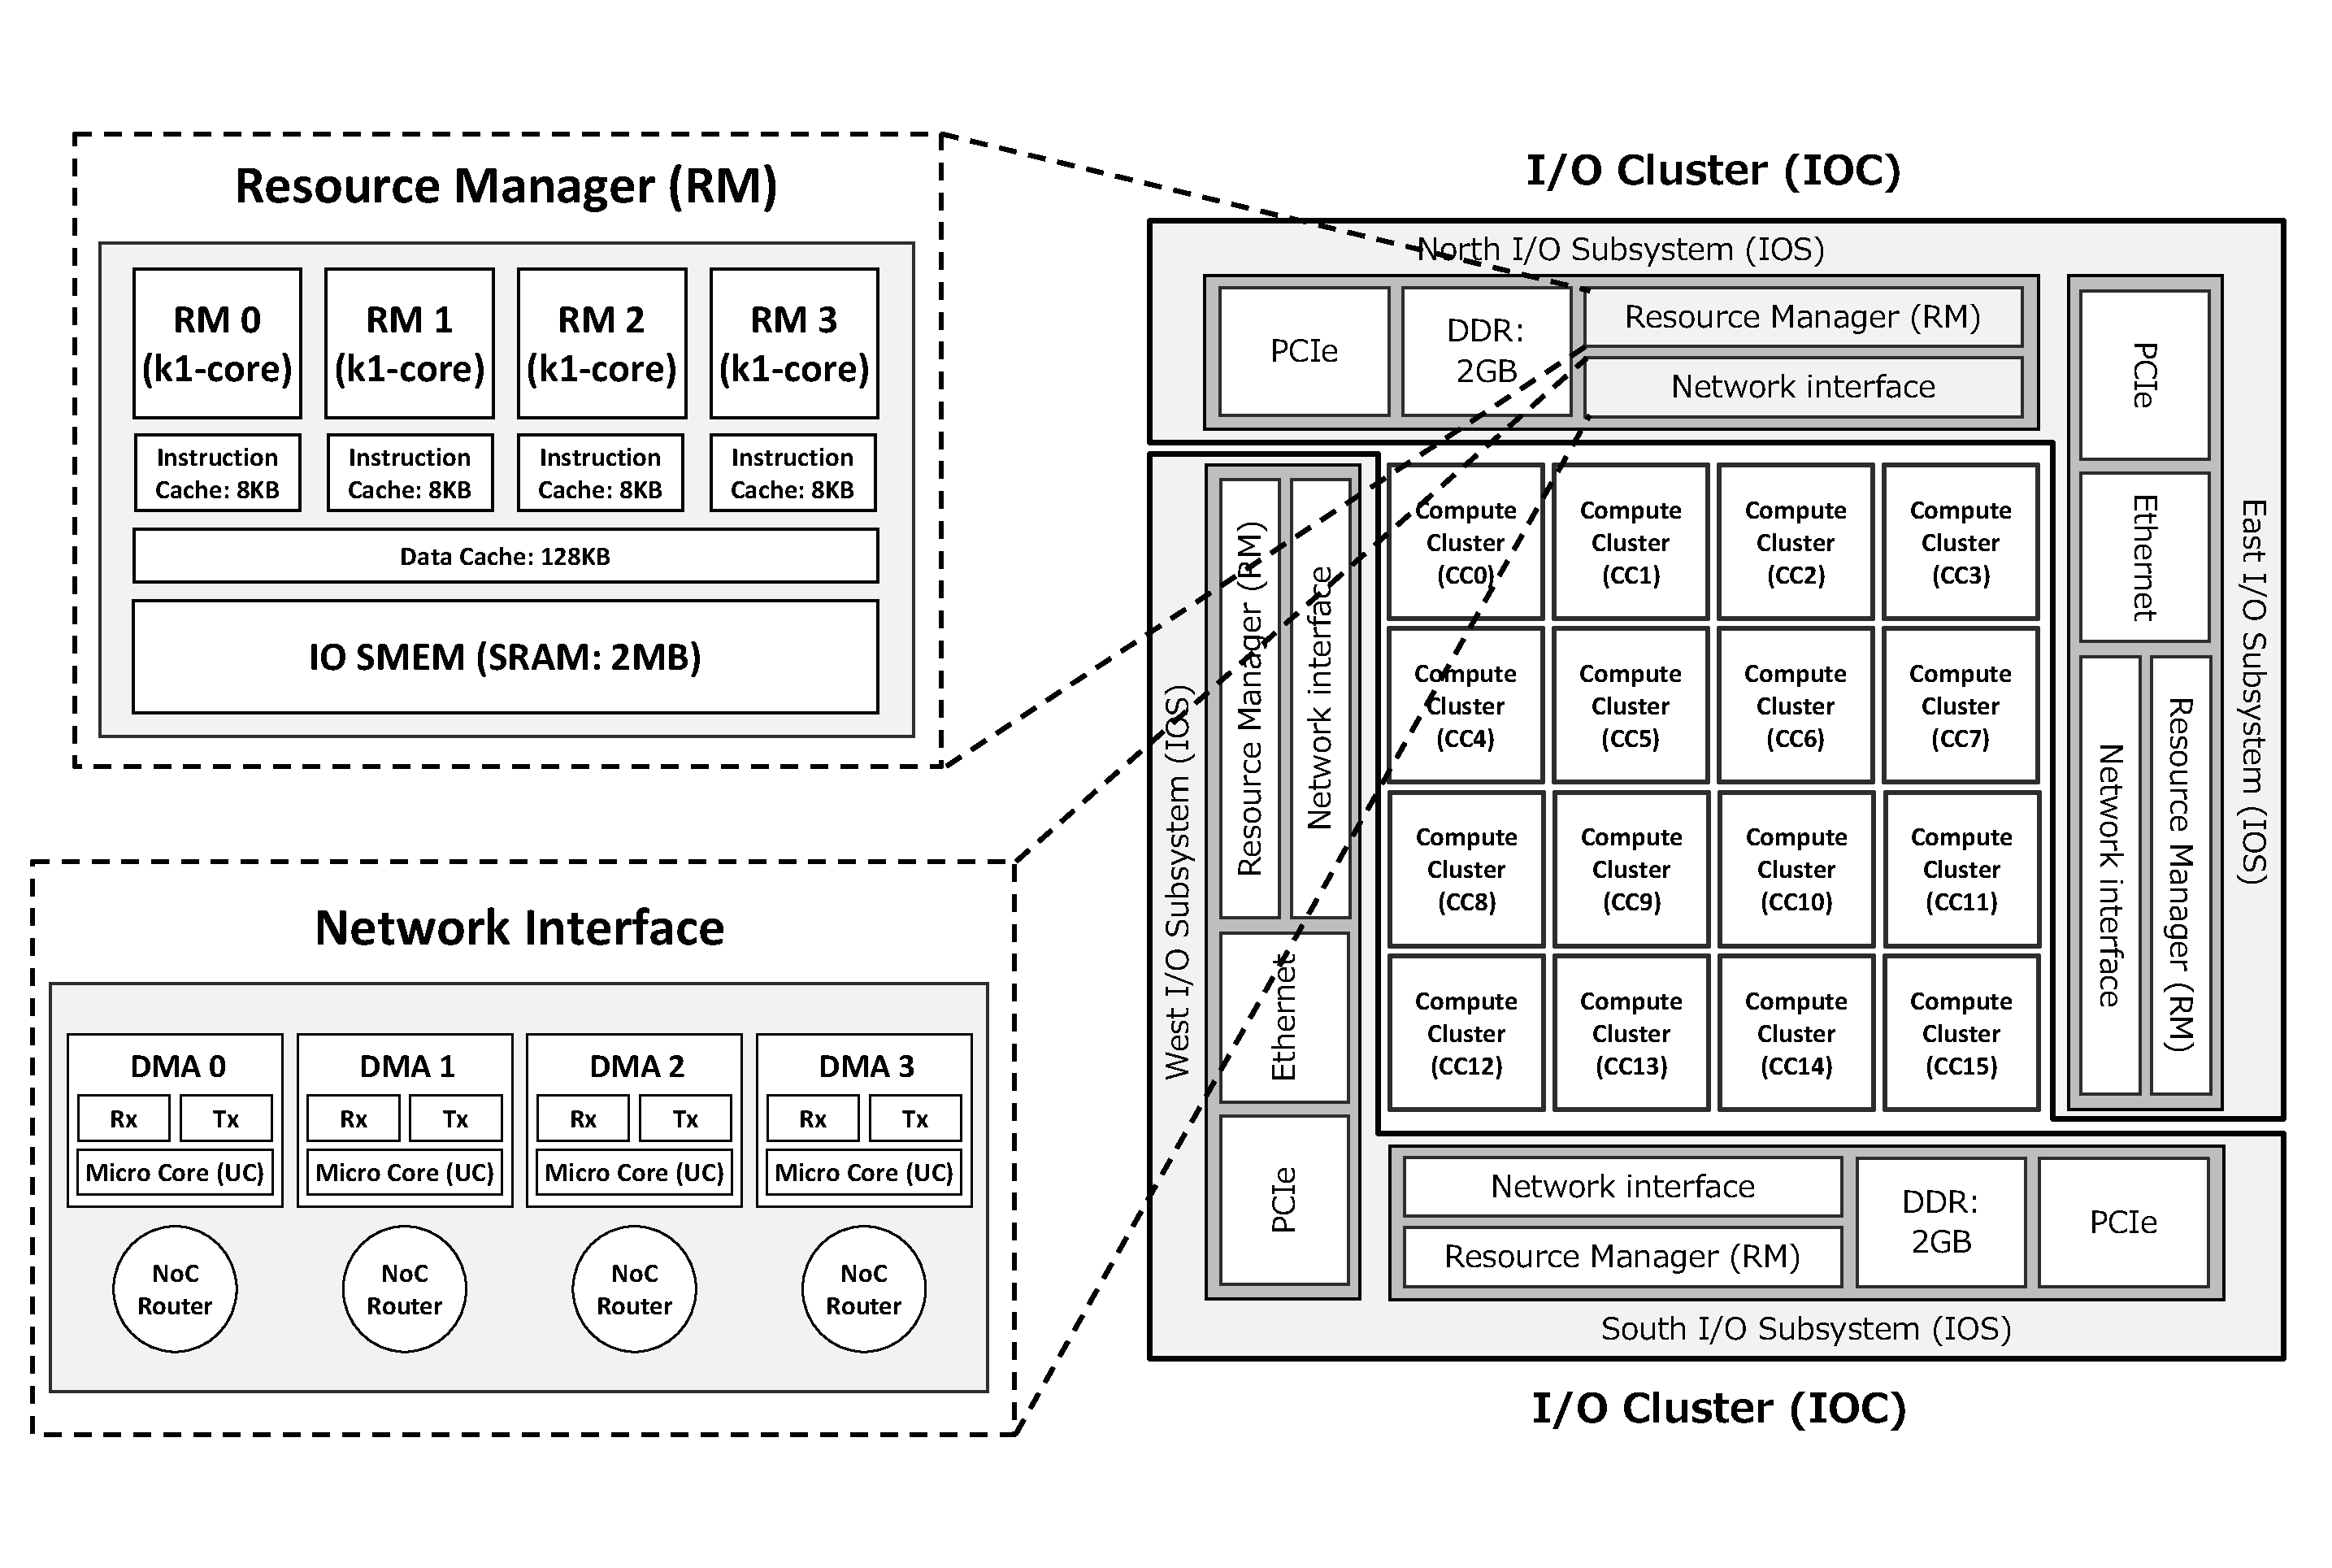
\includegraphics[width=1.0\linewidth]{../figure/mppa_architecture.eps}
  \caption{\label{fig:mppa_architecture}
    Overview of Kalray MPPA-256 Bostan architecture.}
\end{figure}

\subsubsection{Compute Clusters (CC)}
\label{sec:cc}
In MPPA-256, the 16 inner nodes of the NoC correspond to the CCs.
Figure \ref{fig:cc_architecture} illustrates the architecture of each CC.

\begin{itemize}
\item \verb+Processing Elements (PEs) and a Resource Manager (RM)+:
In a CC, 16 processing elements (PEs) and an RM share 2MB cluster local memory (SMEM) composed of 16 independent memory banks of 16 independent memory banks of $16384\times 64 $bit.
Each bank of SMEM has a capacity of 128 KB.
These PEs are mainly used by users for parallel processing.
Developers spawn computing threads on PEs.
The PEs and an RM in CC are the Kalray-1 cores, which implement a 32-bit 5-issue Very Long Instruction Word (VLIW) architecture with 16W-600MHz (typical) or 24W-800MHz.
Each core is fitted with its own instruction and data caches.
Each cache is 2-way associative with a capacity of 8KB.
Thus, 17 k1-cores (a PE or the RM) share multi-banked 2MB SMEM.

\item \verb+A Debug Support Unit (DSU) and a Network Interface+:
In addition to PEs and an RM, bus masters on SMEM are the debug support unit (DSU) and a DMA engine in a network interface.
A DMA engine and a NoC router are laid out in a network interface.
Similar to IOS, the CC DMA engine has also three interfaces: a Rx, Tx, and UC. 
It is instantiated in every cluster and connected to the SMEM.
\end{itemize}

\begin{figure}[t]
  \centering
  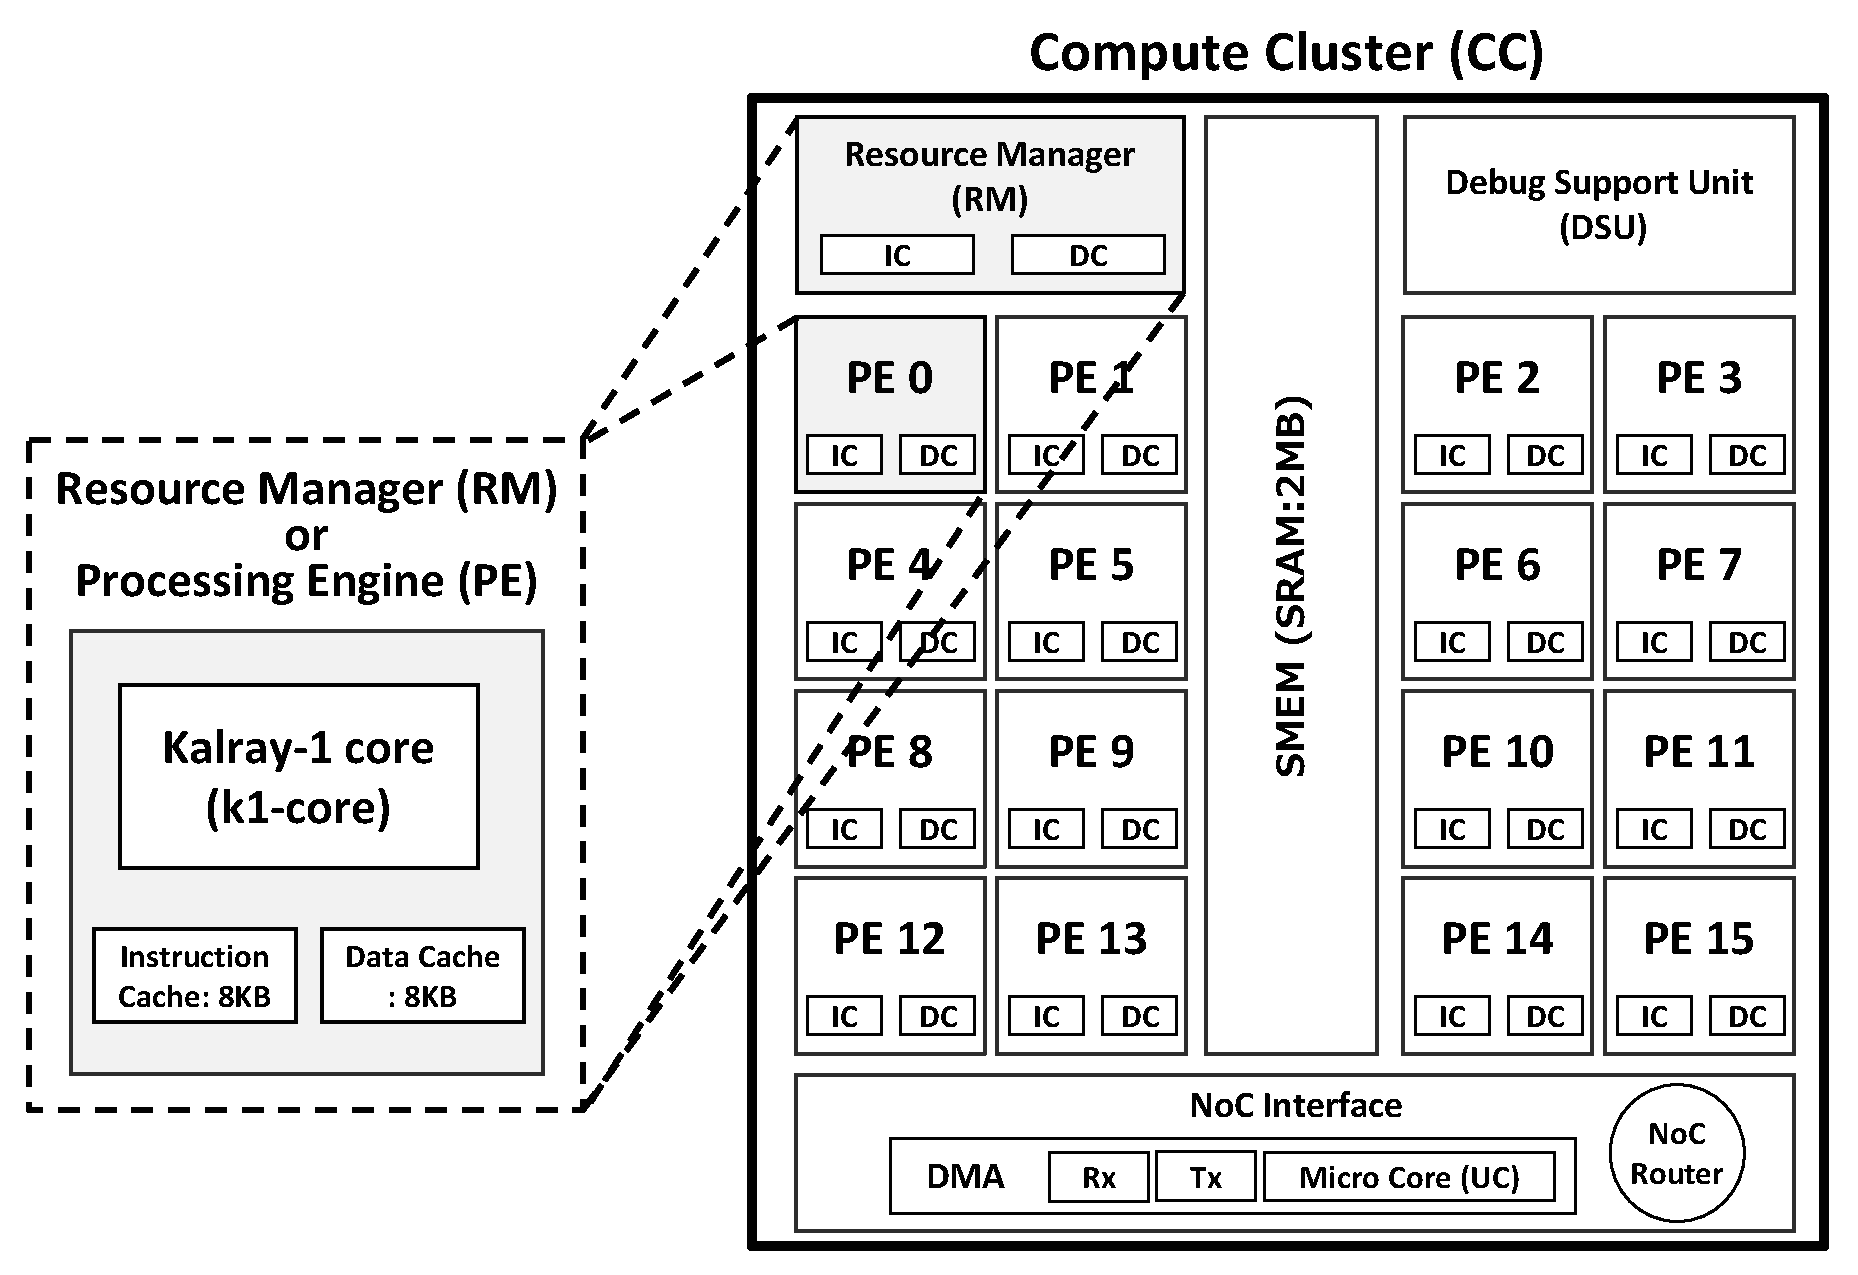
\includegraphics[width=1.0\linewidth]{../figure/cc_architecture.eps}
  \caption{\label{fig:cc_architecture}
    Compute Cluster (CC) architecture.}
\end{figure}


\subsubsection{Network-on-Chip (NoC)}
\label{sec:noc}
The 16 CCs and the 4 IOSs are connected by NoC as shown in Figure \ref{fig:noc_map}.
NoC is constructed on the bus network and routers on each node.

\begin{itemize}
\item \verb+Bus Network+:
Bus network connects nodes (CCs and IOSs) with torus topology \cite{dally2001route}
which has twice band and takes a low average number of hops compared to mesh topology \cite{vangal200780}, \cite{taylor2002raw}.
The network is actually composed two parallel NoC with bi-directional links (red lines in Figure \ref{fig:noc_map}):
the data NoC (D-NoC), which is optimized for bulk data transfers, and the control NoC (C-NoC), which is optimized for small messages at low latency.
Functionally, NoC is a packet switched network.
Data are packaged in variable length packets which circulate between routers in a wormhole manner:
packets are broken into small pieces called flits (flow control digits).
NoC traffic is segmented into packets: each packet has 1 to 4 header flits and 0 to 62 payload data flits.

\item \verb+NoC Routers+:
A node per compute cluster and four nodes per I/O subsystem hold two own routers: a D-NoC router and a C-NoC router
Each RM on NoC node (CC or IOS) is associated with these two NoC routers.
DMA engines in a network interface on CC/IOS send and receive flits through these D-NoC routers with the Rx interface, the Tx interface, and UC.
A mailbox component which is the virtual interface for the C-NoC enables one-to-one, N-to-one, or one-to N low latency synchronizations.
NoC routers shown in Figures \ref{fig:mppa_architecture} and \ref{fig:cc_architecture} illustrate nodes as R0-15, R128-131, R160-163, R224-227, and R192-195 in Figure \ref{fig:noc_map}).
For simplicity, we illustrate D-NoC/C-NoC routers with one NoC router.
In both D-NoC and C-NoC, each network node (CC or IOS) has 5-link NoC routers:
four duplexed links for north/east/west and south neighbours, one duplexed link for local address space attached to the NoC Router.
NoC routers have FIFOs queuing flits for each direction.
The data links are four bytes wide in each direction and operate at the CPU clock rate of 600MHz or 800MHz;
therefore, each tile can transmit/receive a total of 2.4GB/s or 3.2GB/s spread across the four directions (i.e., north, south, east, and west).
\end{itemize}

\begin{figure}[t]
  \centering
  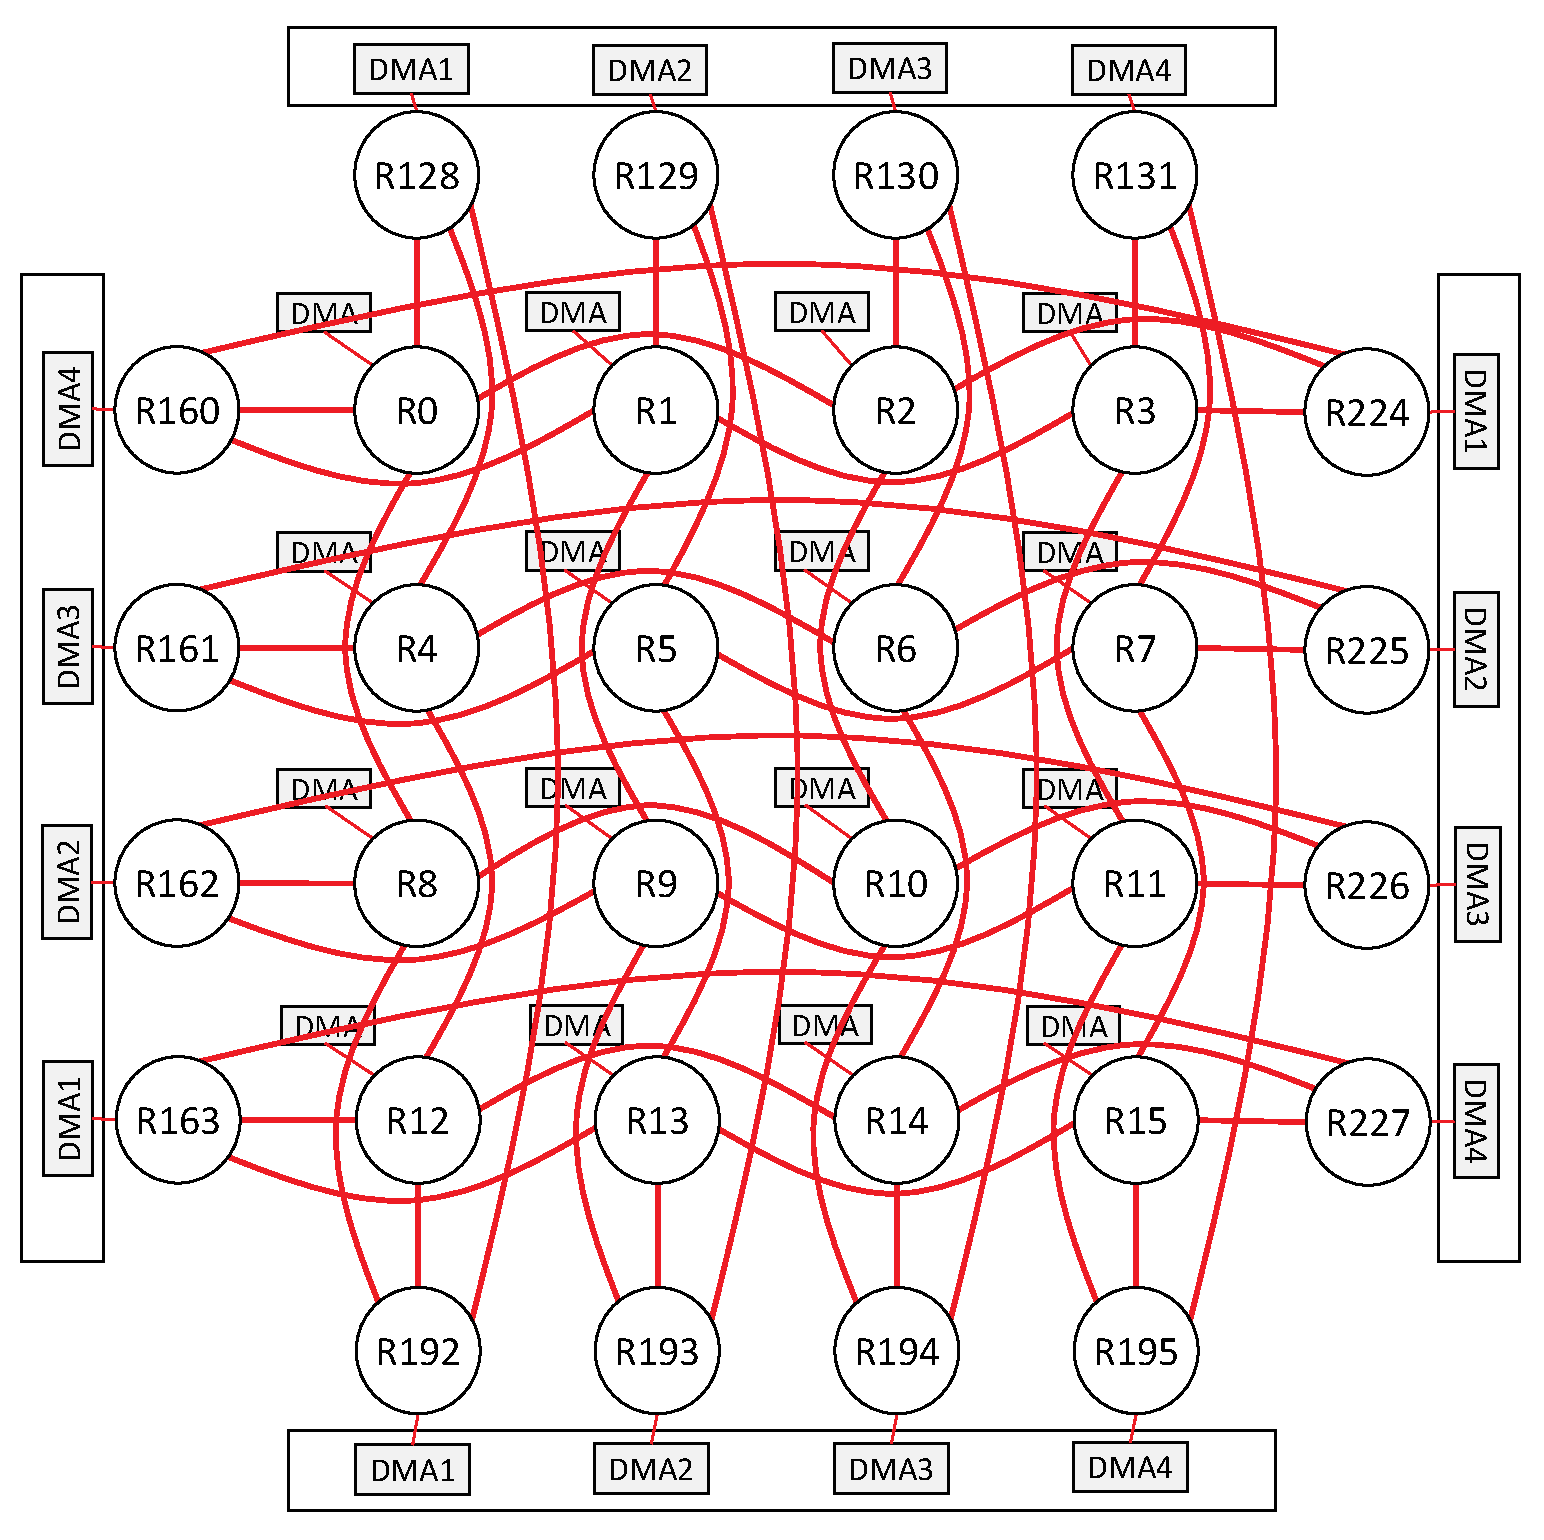
\includegraphics[width=1.0\linewidth]{../figure/noc_map.eps}
  \caption{\label{fig:noc_map}
    Network-on-Chip (NoC) connections (both D-NoC and C-NoC).}
\end{figure}

\subsection{Software model}
\label{sec:software_model}
Software stack for Kalray MPPA-245 used in this paper is shown in Figure \ref{fig:software_stack}.
Kalray's MPPA system is an extensible and scalable array of computing cores and memory.
On such a system, we can map several programming models or runtimes, e.g., Linux, real-time Operating System, POSIX API, OpenCL, OpenMP.
We describe each layer in detail.

In hardware abstraction layer, an abstraction package abstracts hardwares of a CC, IOS, and NoC.
This abstraction package serves as a system that doesn't provide any services.
The hardware abstraction is responsible for partitioning the hardware resources and controlling access to these resources from the user-space operating system libraries.
Moreover, the abstraction package is able to retrieve the resources allocated to a partition at any time.
It is able to set-up and control inter-partition communications as virtual machine abstraction layer.
The hardware abstraction runs on the dedicated RM core.
All the services are commonly provided by a rich operating system (virtual memory, interrupts, scheduler, etc...) must be provided by user-space libraries.
Consequently, each runtime or operating system implements its own required services optimized to its needs.
This is because each programming model or runtime has different requirements.
Minimal kernel avoids the waste of resources and mismatched needs.

In low level Library layer, Kalray also provides libraries for handling NoC.
NoC features such as routing, quality of service are to be set by the programmer.
The Libnoc allows direct access to memory mapped registers for their configurations and use.
It is designed to cause a minimum amount of CPU overhead.
It also serves as a minimal abstraction for resource allocation.
The Librouting offers the minimal set of functions to use for routing data between any clusters of the MPPA,
both with unicast (one target) mode or multicast (multiple targets) mode.
Routing on the torus network shown in Figure \ref{fig:noc_map} is statically conducted with its own policy.
The Libpower enables spawning and waiting for the end of execution of a remote cluster.

In OS layer, various operating systems support the abstraction package.
We introduce the following Real-Time Operating System (RTOS):
\begin{itemize}
\item \verb+RTEMS+: RTEMS, the Real-Time Executive for Multiprocessor Systems, is a full featured RTOS prepared for embedded platforms.
It supports several APIs and standards, and most notably the POSIX API.
The system provides a rich set of features, and an RTEMS application is most of the time just a regular C or C++ program using the POSIX API.
We are able to build RTEMS on IOC.
\item \verb+NodeOS+: On CC, we can build the MPPAcluster operating system a runtime called NodeOS.
This OS addresses the need for a multicore OS conforming as much as possible to the standard POSIX API.
The NodeOS enables user code using POSIX API to run on PEs on CC.
First, NodeOS runtime starts on PE0 before calling the user main function.
Then, we can call \texttt{pthread} on other PEs.
\item \verb+eMCOS+: On both CC and IOS, eMCOS provides minimal programming interfaces and libraries.
eMCOS is a real-time embedded operating system developed by eSOL, a Japanese supplier for RTOS.
eMCOS is the worlds first commercially available many-core RTOS for use in embedded systems.
This OS implements a distributed micro-kernel architecture.
This compact micro-kernel is equipped with only minimal functions.
It enables applications to operate priority based massage passing, local thread scheduling, and thread management on not only IOS but also CC.
\end{itemize}
RTMES and NodeOS are provided by Kalray and eMCOS is released by eSOL.

\begin{figure}[t]
  \centering
  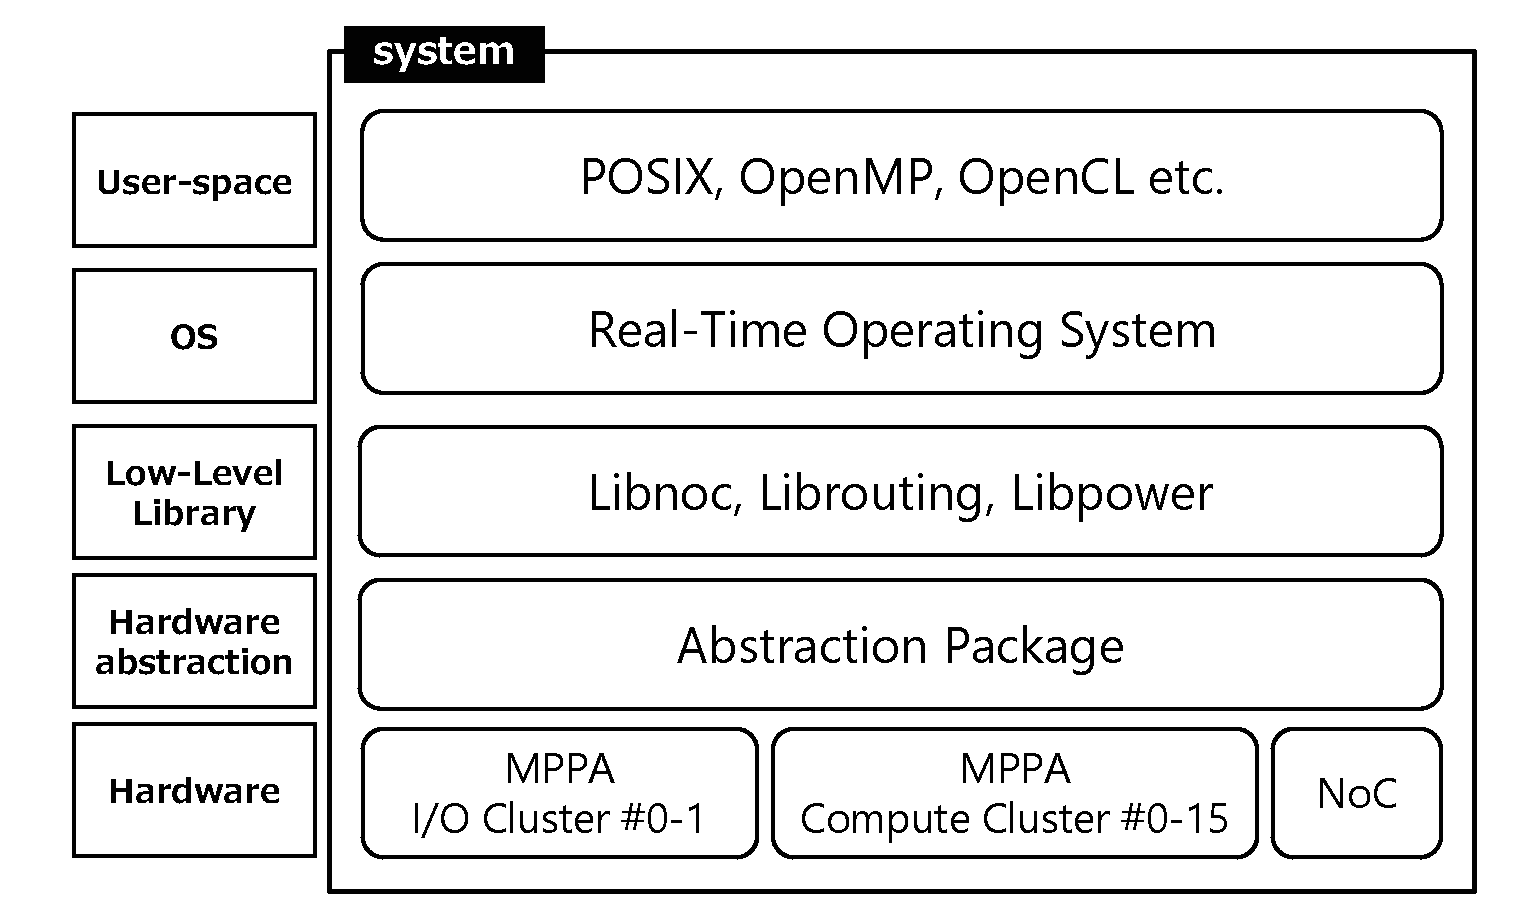
\includegraphics[width=1.0\linewidth]{../figure/softwarestack.eps}
  \caption{\label{fig:software_stack}
    Kalray MPPA-256's software stack.}
\end{figure}


\section{Data Transfer Framework}
\label{sec:framework}


\section{Evaluations}
\label{sec:evaluations}


\section{Related Work}
\label{sec:related work}
In this section, we compare many-core platforms to additional platforms and discuss previous work of multi/many cores.

In recent years, computation performance of a single core processor is constantly coming to its limit.
Pollack has said inefficiency of a single core in \cite{pollack1999new} and Moore's law \cite{moore2006cramming} has become unstable.
To satisfy increasing a demand of computation, CPU is not sufficient.
Many other platforms including many-core are developed and researched nowadays.

Table \ref{tb:comparison_manu-core} summarizes features of many-core platforms with that of other platforms.
For instance, GPU is a powerful device to enhance computing performance.
In specific area (e.g., image processing, learning), it has great potential.
However, it is mainly used for a specific purpose and its reliability is not suitable for real-time systems.
It is difficult to use GPU for a global purpose and a guarantee of reliability due to GPU architecture.
For a global purpose and multiple instructions, many-core is much superior to GPU.
In addition, it is commonly known that many-core has reasonable power consumption.
GPU consumes a lot of power and generates much heat.
This is a critical problem for embedded systems.
DSP and FPGA are also high-performance devices compared to CPU.
They are efficient in a point of power consumption.
DSP is often used for real-time system and FPGA guarantees reliability and efficient processing.
They are suitable for time-critical computing \cite{de2015kalray}.
However, DSP cannot be used for global purpose and programming FPGA is difficult for software developers.
Their software model is much different from CPU and not a substitute for CPU.
Many-core platforms have a potential to take the place of single/multi core CPU.
Ease of programming and scalability with high acceleration is highlighted.

Based on the above background, real-time applications on many-core platforms has received significant attention in recent years.
Many commercial off-the-shelf (COTS) multi-core components are developed and released by several vendors.
(e.g., Kalray's the Multi-Purpose Pro-cessing Array (MPPA) 256 \cite{de2013distributed}, \cite{de2013clustered}, \cite{de2014time},
Intel's Single-chip Cloud Computer (SCC) \cite{intel2015scc},\cite{baron2010single}, Tilera's Tile64 \cite{tilera2015tile64}, and
Intel's Xeon Phi \cite{chrysos2014intel} \cite{chrysos2012intel})
The Kalray MPPA-256 is designed for real-time embedded applications and the target of this paper.
Kalray S.A \cite{de2013distributed}, \cite{de2013clustered}, \cite{de2014time} has presented clustered many-core architectures on NoC.
(Precise hardware model is described in Section \ref{sec:hardware_model}.)
It is often accepted for a target of many-core platforms and various previous work has considered this model \cite{perret2016temporal}, \cite{becker2016contention}, \cite{carle2014static}, \cite{perret2016mapping}.


In \cite{saidi2015shift}, many opportunities and challenges of multi/many core platforms are discussed.

[note]

disussion: \cite{saidi2015shift}

mppa:
  architecture \cite{de2013distributed}, \cite{de2013clustered}, \cite{de2014time},
  report \cite{kanter2015kalray}, 
  slide(DSP->many-core) \cite{de2015kalray},  
  NoC \cite{denet2017work}, \cite{deDinechin2014GSN},

mapping: \cite{perret2016mapping}(DAG), \cite{puffitsch2015off}, \cite{carle2014static}, \cite{becker2014mapping}, \cite{faragardi2014communication}

memory: \cite{perret2016predictable}, \cite{becker2016contention}

AUTOSAR mapping: \cite{becker2016contention}, \cite{faragardi2014communication}

aircraft(airbus): \cite{perret2016temporal}, \cite{perret2016predictable}, \cite{perret2016mapping}. 

\renewcommand{\arraystretch}{2.0}
\begin{table*}[t]
  \caption{\label{tb:comparison_manu-core}
    Comparison of Many-core to CPU, GPU, DSP, and FPGA}
  \centering
  \scriptsize	                    % text size
  \tabcolsep = 1.5mm              % side-margin in column
  \begin{tabular}{c|cccccccccc}
    \hline
    & \multirow{2}{*}{\textbf{performance}} & \multirow{2}{*}{\textbf{power/heat}} & \multirow{2}{*}{\textbf{reliability}} & \multirow{2}{*}{\textbf{real-time}} & \textbf{software} & \multirow{2}{*}{\textbf{costs}} & \textbf{multiple}\\
    &&&&& \textbf{development} && \textbf{instruction} \\
    \hline
    \hline
    CPU & & \(\bigtriangleup\) & \(\checkmark\) & \(\checkmark\) & \(\checkmark\) & \(\checkmark\) & \(\bigtriangleup\) \\
    GPU & \(\checkmark\) &  & \(\bigtriangleup\) &  & \(\bigtriangleup\) & \(\checkmark\)\\
    DSP & \(\bigtriangleup\) & \(\bigtriangleup\) & \(\checkmark\) & \(\checkmark\) & \(\bigtriangleup\) & \(\checkmark\) & \\
    FPGA & \(\checkmark\) & \(\bigtriangleup\) & \(\checkmark\) & \(\bigtriangleup\) &  & \(\bigtriangleup\) & \\
    Many-core & \(\checkmark\) & \(\checkmark\) & \(\checkmark\) & \(\checkmark\) & \(\checkmark\) & \(\bigtriangleup\) & \(\checkmark\) \\
    \hline
  \end{tabular}
  \vspace{-5mm}
\end{table*}


\renewcommand{\arraystretch}{2.0}
\begin{table*}[t]
  \caption{\label{tb:comparison_relatedwork}
    Comparison to Related Work}
  \centering
  \scriptsize	                    % text size
  \tabcolsep = 1.5mm              % side-margin in column
  \begin{tabular}{c|ccccccccc}
    \hline
    &  &  &  &  &  & \\
    \hline
    \hline
    \cite{saidi2015shift} &  &  &  &  &  & \\
    \cite{perret2016mapping} &  &  &  &  &  & \\
    \cite{becker2016contention} &  &  &  &  &  & \\
    this paper &  &  &  &  &  & \\
    \hline
  \end{tabular}
  \vspace{-5mm}
\end{table*}


\section{Conclusion}
\label{sec:conclusion}

[note]
future work: \cite{maruyama2016ros2}


%%
\bibliographystyle{abbrv}       % ACM
\bibliography{reference}

\end{document}

